\eat{
\begin{figure*}[tb!]
\vspace{-2ex}
\begin{minipage}[t]{0.5\textwidth}
\begin{center}
\subfigure[{\scriptsize TWPageRank (batch vs. inc.)}]{\label{fig-aminer-time2}
\includegraphics[scale=0.38]{./exp/AMiner_time_twpr.eps}}
%\quad\quad
\hspace{-0.5ex}
\subfigure[{\scriptsize Comparison of ranking algorithms}]{\label{fig-aminer-time1}
\includegraphics[scale=0.38]{./exp/AMiner_time.eps}}
\end{center}
\vspace{-5ex}
\caption{\small Efficiency tests on \aminer}
\label{fig-aminer-time}
\end{minipage}
\hspace{-2ex}
\begin{minipage}[t]{0.5\textwidth}
\begin{center}
\subfigure[{\scriptsize \aminer}]{\label{fig-aminer-time-sigma}
\includegraphics[scale=0.38]{./exp/AMiner_sigma_time.eps}}
%\quad\quad
\hspace{-0.5ex}
\subfigure[{\scriptsize \magdata}]{\label{fig-mag-time-sigma}
\includegraphics[scale=0.38]{./exp/MAG_sigma_time.eps}}
\end{center}
\vspace{-5ex}
\caption{\small Efficiency tests: varying $\sigma$}
\label{fig-time-sigma}
\end{minipage}
\vspace{-1ex}
\end{figure*}
}

\newcommand{\graphscaleexpapp}{0.262}
\newcommand{\graphmarginexpapp}{-2ex}
%%% all in 1 Figure
\begin{figure*}[tb!]
%\vspace{-2ex}
\begin{center}
%\hspace{-10ex}
\subfigure[{\scriptsize \aan}]{\label{fig-aan-ab-recom}
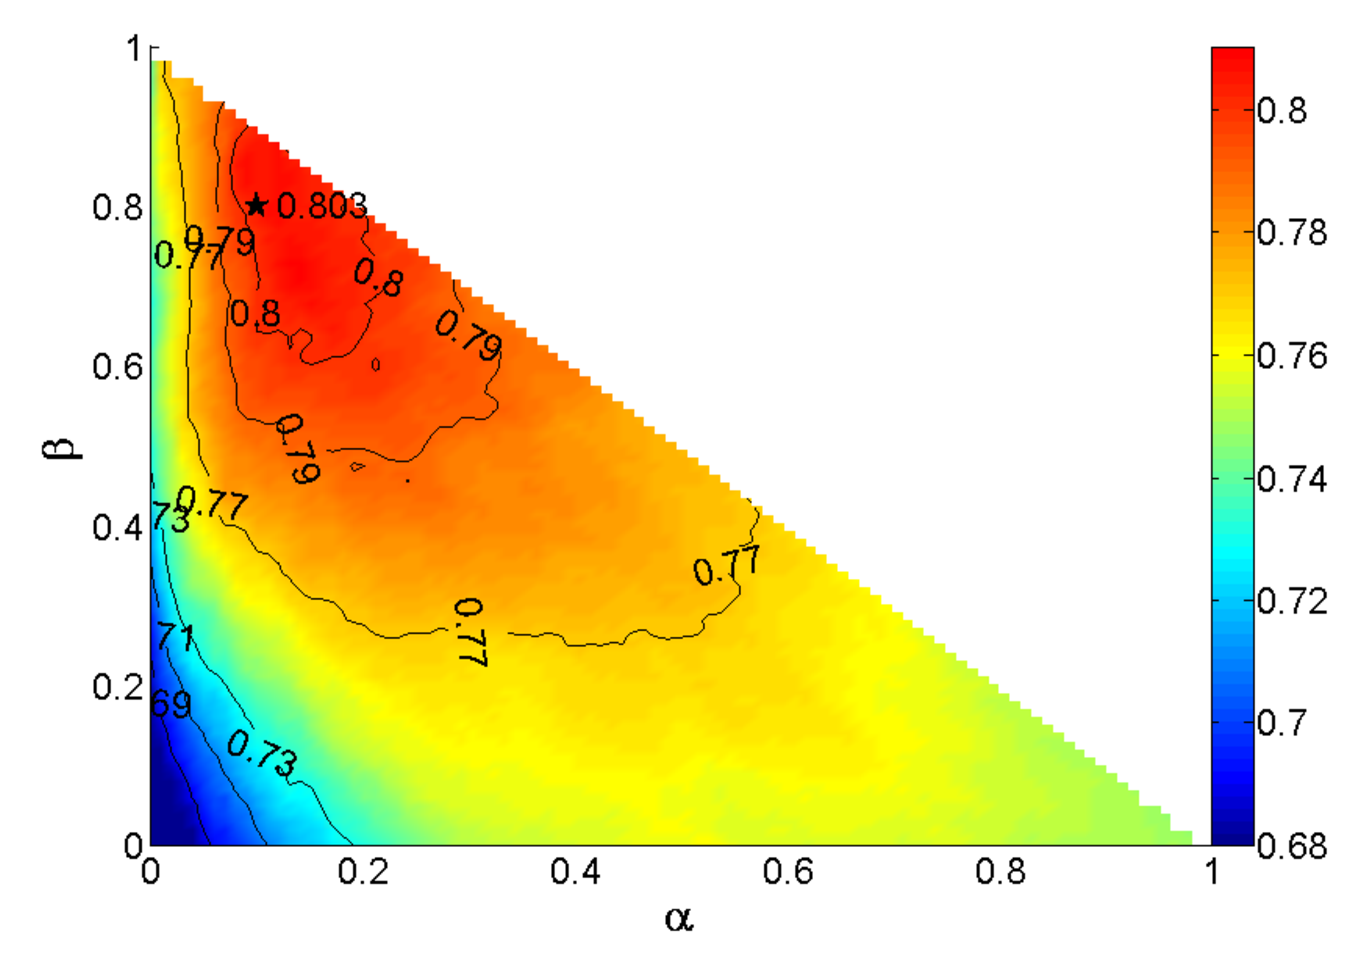
\includegraphics[scale=\graphscaleexpapp]{./exp/AAN-para-recm.eps}}
%\quad\quad
\hspace{\graphmarginexpapp}
\subfigure[{\scriptsize \aminer}]{\label{fig-aminer-ab-recom}
\includegraphics[scale=\graphscaleexpapp]{./exp/AMiner-para-recm.eps}}
%\quad\quad
\hspace{\graphmarginexpapp}
\subfigure[{\scriptsize \magdata}]{\label{fig-mag-ab-recom}
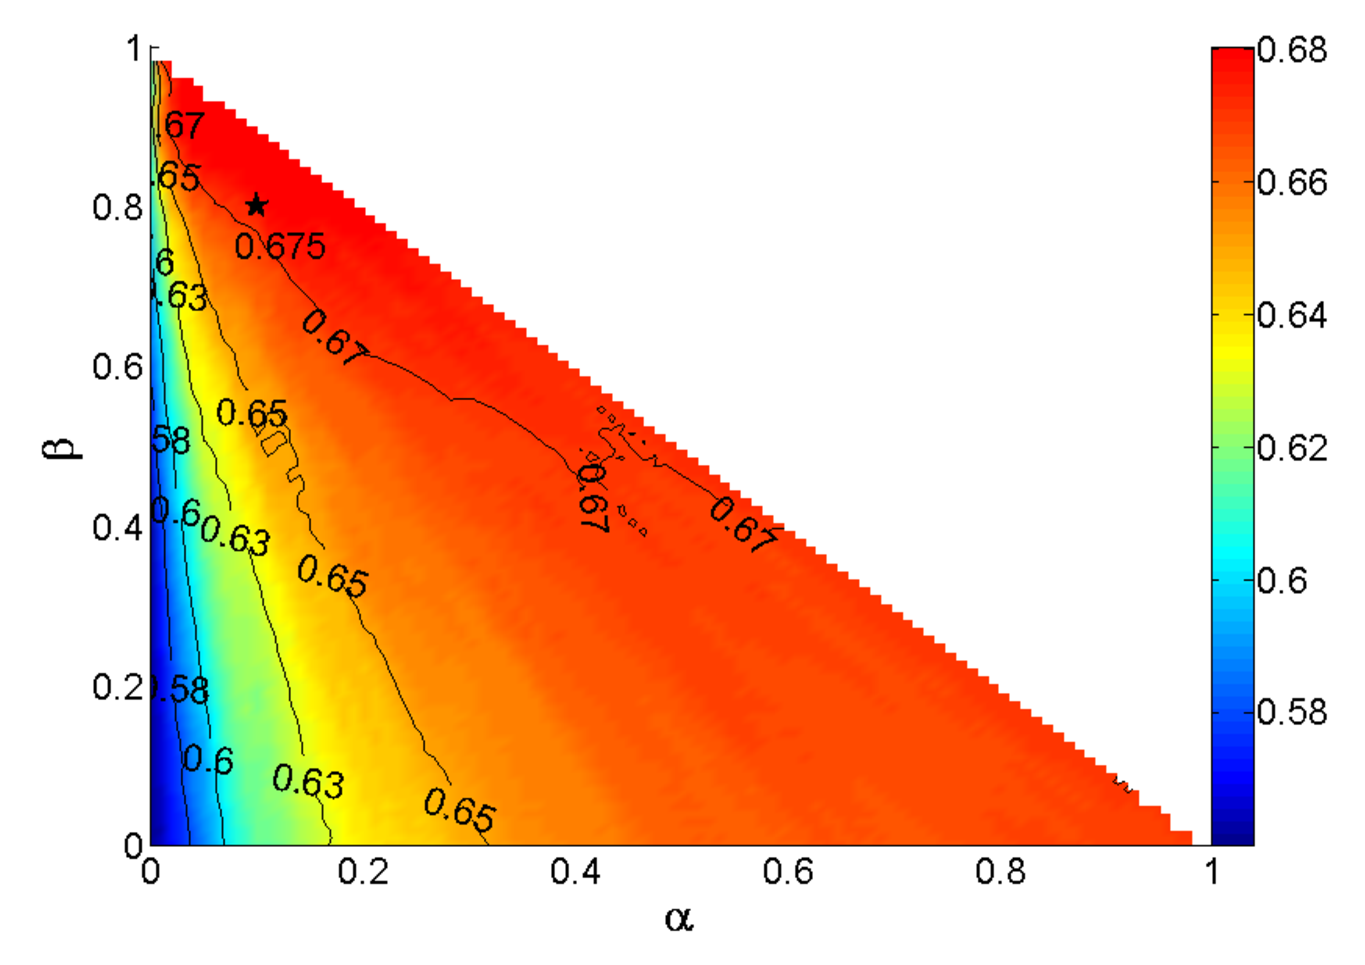
\includegraphics[scale=\graphscaleexpapp]{./exp/MAG-para-recm.eps}}
\\ %%%%%%%%%%%%%%%%%%%%%%%%%%%%%%%%%%%%%%
\vspace{-3ex}
%\hspace{-10ex}
\subfigure[{\scriptsize \aan}]{\label{fig-aan-ab-fcita}
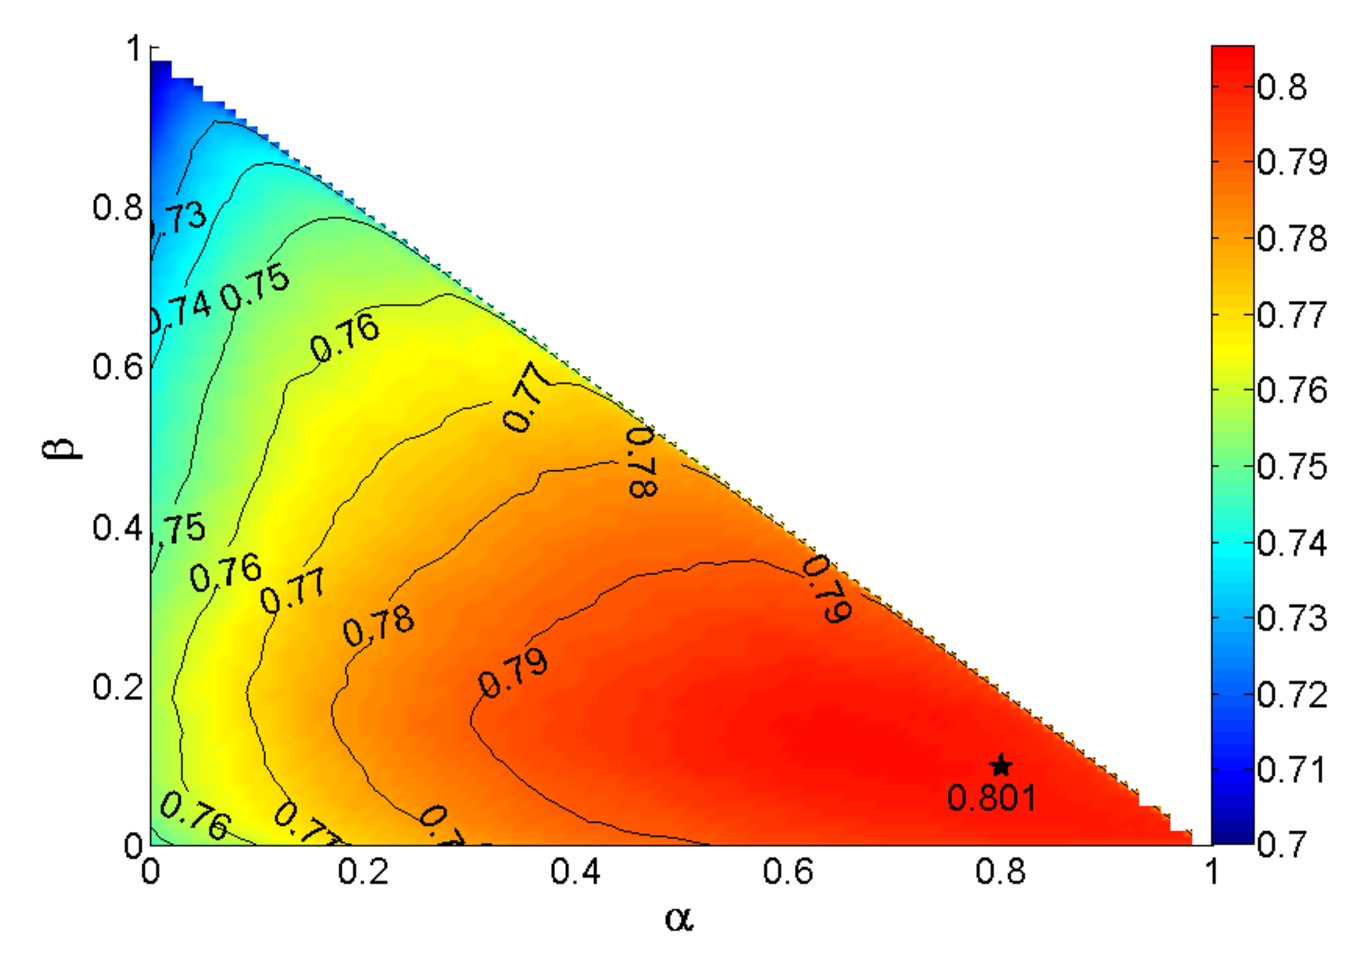
\includegraphics[scale=\graphscaleexpapp]{./exp/AAN-para-fcita.eps}}
%\quad\quad
\hspace{\graphmarginexpapp}
\subfigure[{\scriptsize \aminer}]{\label{fig-aminer-ab-fcita}
\includegraphics[scale=\graphscaleexpapp]{./exp/AMiner-para-fcita.eps}}
%\quad\quad
\hspace{\graphmarginexpapp}
\subfigure[{\scriptsize \magdata}]{\label{fig-mag-ab-fcita}
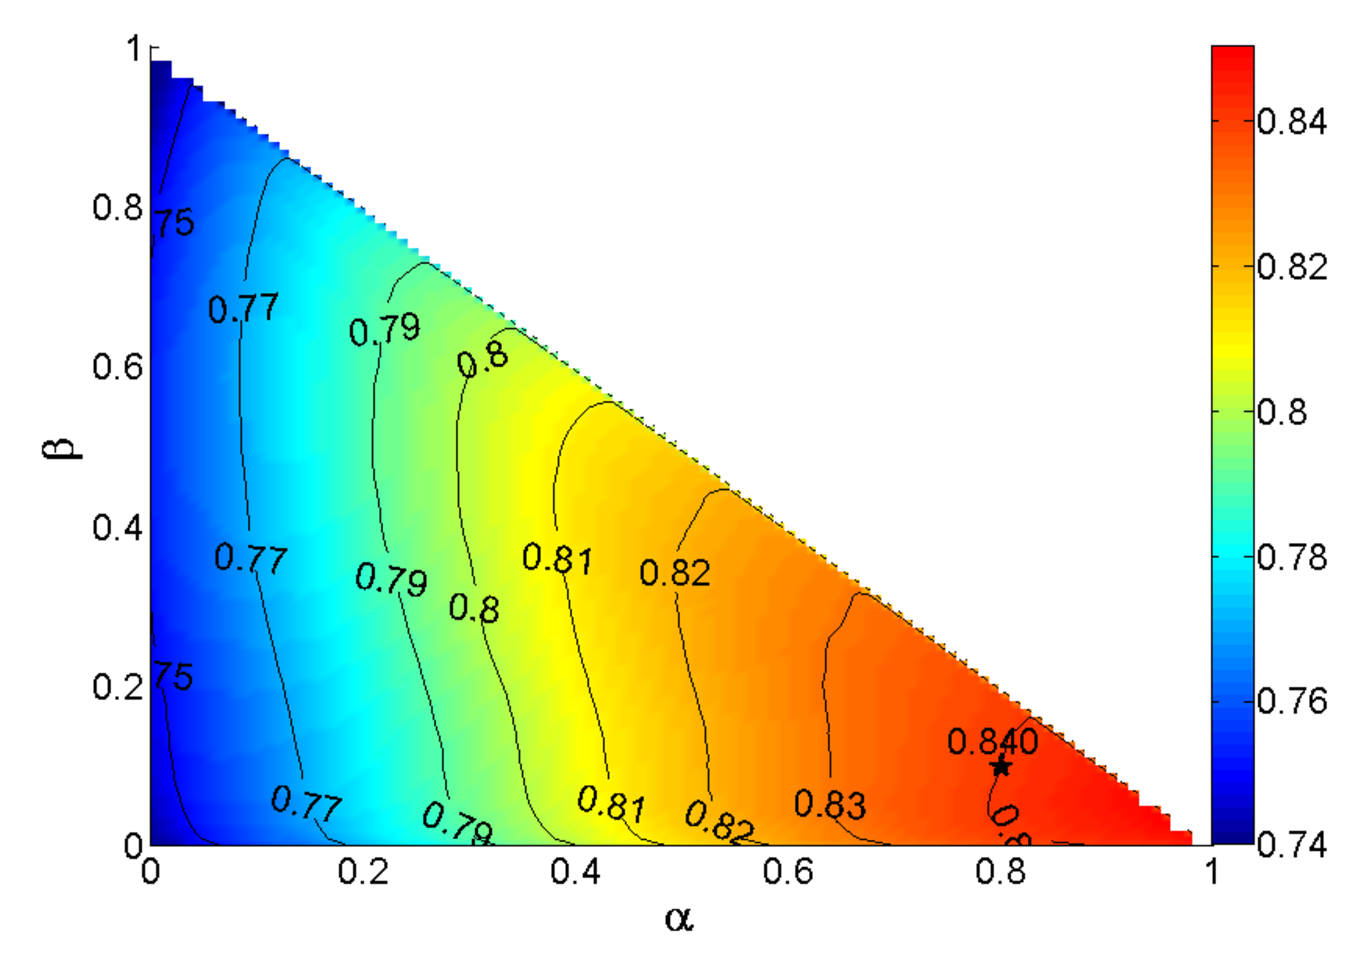
\includegraphics[scale=\graphscaleexpapp]{./exp/MAG-para-fcita.eps}}
\end{center}
\vspace{-5ex}
\caption{\small Accuracy tests with \recom ((a)--(c)) and \fcita ((d)--(f)): varying aggregating parameters $\alpha$ and $\beta$}
\label{fig-ab}
\vspace{-3ex}
\end{figure*}
%%%%%%%%%%%%%%%%%%%%%%%%%%%%%%%%%%%%%%

\vspace{-1ex}
\section*{APPENDIX A: Further Experiments}
\label{sec-exp-app}

\subsection*{1. Detailed results of Exp-4.3} %$\alpha$ and $\beta$ (detailed)

%We present detailed results of {\em Exp-4.3}, which are omitted earlier due to the space constraints, \ie the impacts of aggregating parameters $\alpha$ and $\beta$ on effectiveness.

\eat{
\etitle{Exp-4.1}. To evaluate the impacts of the time decaying factor $\sigma$, we varied $\sigma$ from -1.6 to -0.4, while fixed $Y_s$ to default values, $b=+\infty$ and $dif=1$. The efficiency results are reported in Fig.~\ref{fig-time-sigma}.
Note that the running time of algorithm \batensemble is different on \recom and \fcita because of the different splitting year $Y_s$.

When varying $\sigma$, the running time of \batensemble is almost stable on both \aminer and \magdata using \fcita and \recom. Indeed, the running time using (\fcita, \recom) only varies (1.4\%, 0.5\%) on \aminer, and (2.1\%, 2.2\%) on \magdata, on average, respectively.
}

\etitle{Exp-4.3}.
To evaluate the impacts of aggregating parameters $\alpha$ and $\beta$, we varied $\alpha$ and $\beta$ at the granularity of 0.01.
The results are reported in Fig.~\ref{fig-ab}, where the parameters selected earlier and their corresponding \PairAcc are marked with $*$.

When varying $\alpha$ and $\beta$, the \PairAcc of \ensemblerank changes gently, as shown in Fig.~\ref{fig-ab}.
The optimal \PairAcc is obtained within a single region, rather than a complex collection of optimal regions.
%
Moreover, the \PairAcc keeps at a high level within a certain ($\alpha$, $\beta$) combination space around the optimal region, as shown in Fig.~\ref{fig-ab}.
%For instance, consider a square of length 0.3, which covers 8.5\% of the parameter combination space. The fraction of parameters such that the \PairAcc is no worse than 1\% of the corresponding \PairAcc with marker $*$ is (73\%, 94\%) on \aan, (96\%, 87\%) on \aminer and (83\%, 95\%) on \magdata, using (\recom, \fcita), respectively.
%
Further, the optimal parameters on the same benchmarks are very similar for (\aan, \aminer and \magdata), indicating that the setting of $\alpha$ and $\beta$ can be easily transferred across different datasets.
To conclude, \ensemblerank is very robust to parameters $\alpha$ and $\beta$, and it is quite flexible for choosing proper values of parameters $\alpha$ and $\beta$.

Moreover, varying $\alpha$ and $\beta$ also enables to verify the effectiveness of importance assembling from multiple components.
And the ranking based on all components consistently performs the best, which, using \recom and \fcita, improves the \PairAcc over using components (C, V, A, CV, CA, VA) by (6.33\%, 19.4\%, 16.3\%, 0.33\%, 4.97\%, 6.33\%) and (9.58\%, 23.8\%, 5.98\%, 2.56\%, 0.74\%, 4.82\%) on \aan, (3.21\%, 23.9\%, 15.1\%, 0.93\%, 1.66\%, 7.97\%) and (16.8\%, 12.5\%, 9.60\%, 0.34\%, 1.87\%, 6.37\%) on \aminer, and ( 2.43\%, 16.0\%, 14.2\%, 0.05\%, 2.38\%, 5.38\%) and (8.89\%, 19.3\%, 11.2\%, 1.43\%, 0.77\%, 9.65\%) on \magdata, respectively.

